\chapter{Overview} \label{cap:overview}

\section{The Big Picture - the Overall Architecture [Herbert]}
The following subsections are aiming on providing a rough overview on the
componentes of the Insieme project.

\subsection{The Compiler and the Runtime}
The Insieme project comprises two major components -- the \textit{Insieme
Compiler} and the \textit{Insieme Runtime}. The compiler's task is to convert
input codes based on various languages (C, C++, OpenCL) into a C-based
representation which, combined with the Runtime, can be compiled into a binary
exhibiting the behaviour as intended by the programmer of the input program.
During this process, the compiler is allowed to analyse, manipulate and
restructure the handled code (fragment) as long as the \textit{intended}
semantic of the program is not lost. Some of these transformations may include
look restructuring or reordering, optimization of message passing operations,
array manipulations, the introduction or elimination of parallel constructs or
the conversion of originally C based codes into OpenCL. 

The \textit{Runtime's} contribution on the other hand is to provide an abstract
interface to the underlying hardware infrastructure. It therefore requires the
handled program to follow a specific application model, allowing the runtime to
inspect and steer the execution of the corresponding code. In particular, all
codes to be executed using the runtime have to be organized within \textit{work
items}. \index{Work Items} Essentially, a work item is a piece of code that can
be invoked by providing the required input data -- similar to procedures.
However, work-items have a fixed signature, hence all of them can be generically
invoked by the runtime. Further, for each of those, meta information regarding
the accepted input-parameters is offered within a table, the
\textit{implementation table}. Furthermore, unlike ordinary procedures, the
work-load of a single invocation may be shared among multiple threads. The exact
number can be determined by the runtime. The work-item implementation will use
those threads to conduct its task efficiently. Last but not least, each
work-item can offer multiple implementations -- each specialized for particular
scenarios -- to the runtime. One implementation may be chosen for a serial
execution, not including any synchronization primitives. Another may be used for
conducting the computation on an accelerator. The characteristic of the offered
implementations is described by additional meta-information offered within the
\textit{implementation table}.

Although the Compiler is supporting other output formats too (e.g. plain
sequential C code), the ``native'' backend of the compiler is generating code
fitting the requirements of the runtime. Therefore the code is decomposed
into work-items and the required meta-information is collected via static code
analyses and stored within the corresponding \textit{implementation table}.

Form the Insieme developers point of view the Compiler and Runtime are
practically two different worlds. For once, the Compiler is implemented using
C++11 while the Runtime is based on C99. Furthermore, the Compiler constitutes a
library of passive functions to be orchestrated by the developer while the
runtime is a framework. Further general information regarding these two major
components will be covered within the following subsections. A detailed
coverage of the Compiler components can be found within chapter
\ref{cap:compiler} and for the Runtime within chapter \ref{cap:runtime}.


\subsection{The Compiler}

\subsubsection{The Obligation}
The compiler provides a set of libraries including algorithms and data
structures to load, parse, analyses, manipulate and synthesize programs. Its
major obligation is to provide these set of tools, enabling the research in
static program optimization. Furthermore, utilities supporting the
instrumentation, generation, compilation, (remote) execution and collection of
measurement results are supported \ref{sec:Driver.MeasureAndInstrument}. Hence,
the otherwise static part of the compiler can incorporate dynamic code
properties if desired.

A related requirement to the compiler is the desire of using the available
utilities as flexible as possible. Developers aiming on conducting compiler
research shell be enabled to easily combine the available means according to
their own requirements. To support this, all modules are required to deal with a
consistent data format used for representing the processed program code.
Consequently, a common internal representation for processed code is among the
most essential components of the compiler. In fact, it is forming the
centerpiece of the entire compiler infrastructure.

The Insieme parallel intermediate representation (INSPIRE or just IR if the
context is clear) is realizing this central component. This formal language has
been designed to express parallel concepts encountered within parallel
programming languages like OpenMP, OpenCL and MPI in a uniform way. The key idea
of the compiler is to convert all supported input languages into this unified,
streamlined IR. This way, for the compiler researcher focusing on improving
optimization in the context of parallel applications, this unified view provides
the benefit of already resolved ambiguities present within the input languages.
For researches being interested in a single input language this common internal
core ensures that similar utilities developed for related problems encountered
within other languages can be re-used. For instance, the extraction of a
parallel control flow graphs and algorithms operating on them
originally developed for analysing MPI codes can be reused for research on
OpenMP and OpenCL codes if required.\note{the pCFG has not yet been implemented}

Bottom-line -- the compiler is providing the means to represent parallel
programs as well as utilities to derive them from input codes, analyse and
manipulate them and finally modules converting the internal representation into
some form of processable output code (typically C). On top of this, a set of
utilities performing higher level functions like generic optimizations or
parameter studies are offered. All those are offered to provide an
infrastructure for compiler research on parallel codes.

\subsubsection{The Application Model}
As has been stated within the previous section, the internal application model
used to represent and process programs throughout the compiler is INSPIRE. It
represents applications based on an execution-oriented (in contrast to a
syntax-oriented) way. Hence, the actual execution should be modeled, not the
structure of the original code describing this execution. The IR offers basic
imperative structures including ordinary statements, conditions, switches,
for- and while-loops. However, functional concepts including higher-level
functions and lambdas are as well supported. Those features have especially been
included to support the recursive composition of arbitrary program constructs.
This should prevent the future need for extending the language. Every future
extensions should be supportable by combining existing constructs using
functional composition. The goal is to keep the language core as closed as
possible such that tools relying on those constructs need not be updated in case
new constructs are introduced over time.

Additionally, the IR has been designed to simplify analyses. The IR is kept
minimal and compact. Hence, only a small (yet not minimal due to concessions
toward intuitiveness) number of constructs are used to represent a program.
Details covering semantically irrelevant concepts like names of variables or
functions are as well discarded as the formatting of the input code. This way,
analyses can focus on the essential parts. The additional explicit
representation and unification of concepts like direct / indirect memory
accesses, memory management and parallelism (should) simplify the design and
implementation of code analyses. \note{at this stage, the development in this
direction hasn't reached a state to state consequences of the IR on the analyses
with absolute certainty} Much more details on the Insieme IR can be found within
the INSPIRE language specification \cite{insieme_ir_spec}.


\subsubsection{Important Components}

\begin{figure}[tb]
	\centering
	%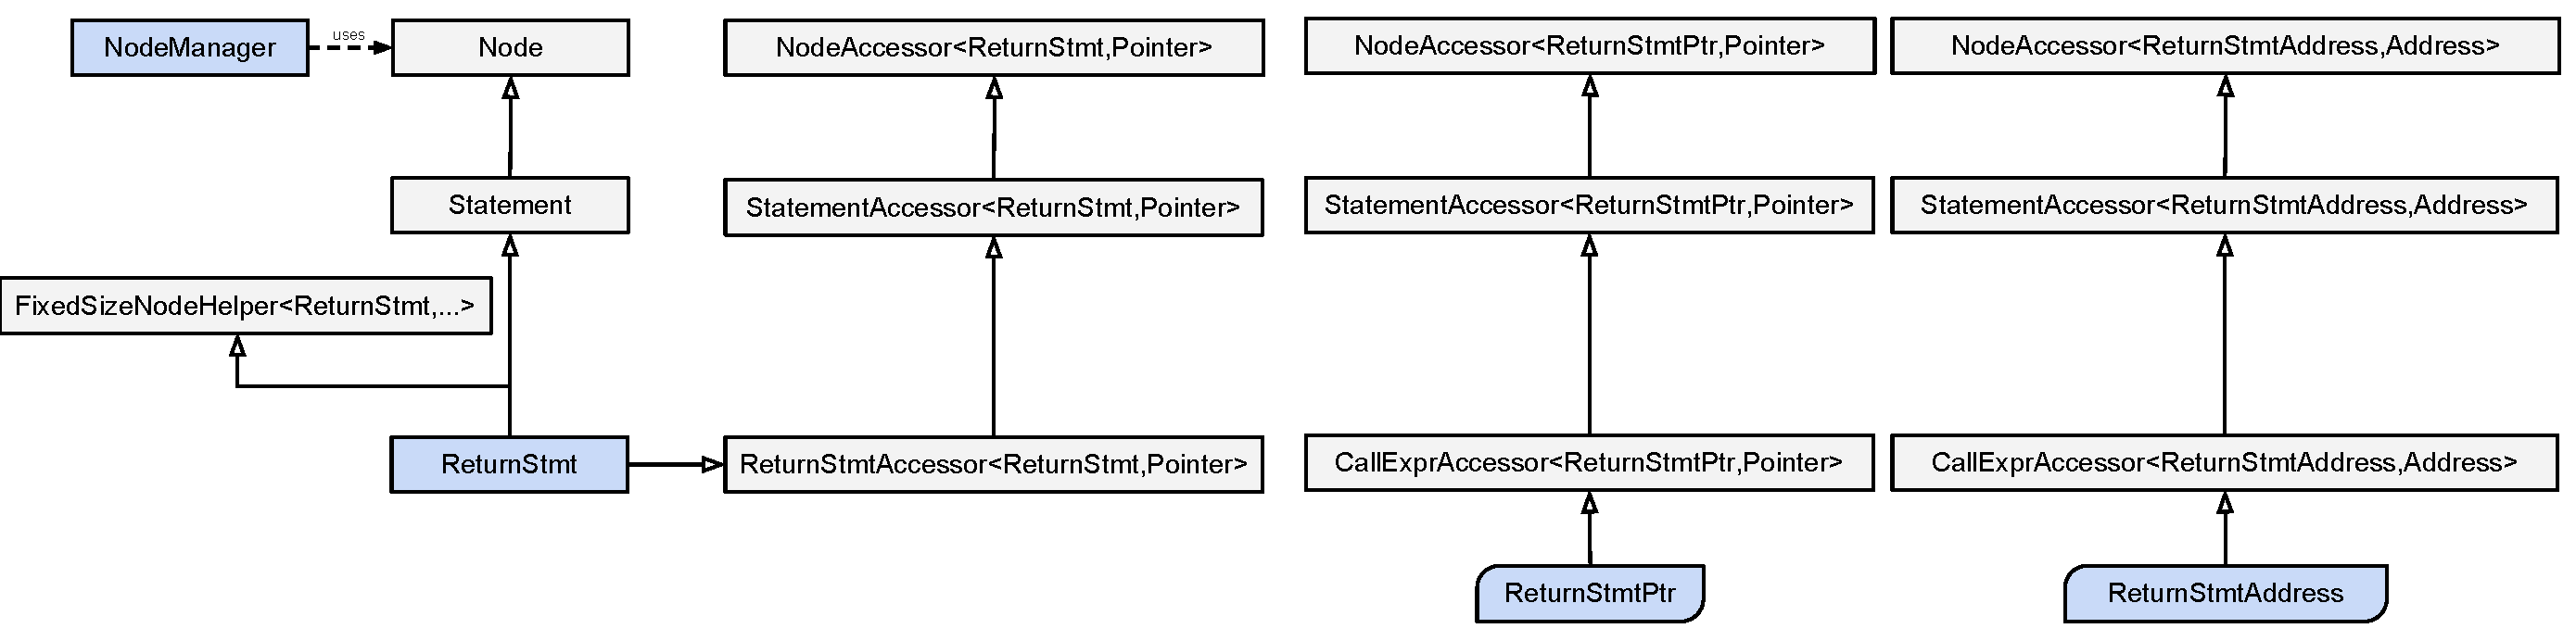
\includegraphics[width=\textwidth]{compiler/core/class_hierarchy_of_return_stmt.pdf}
	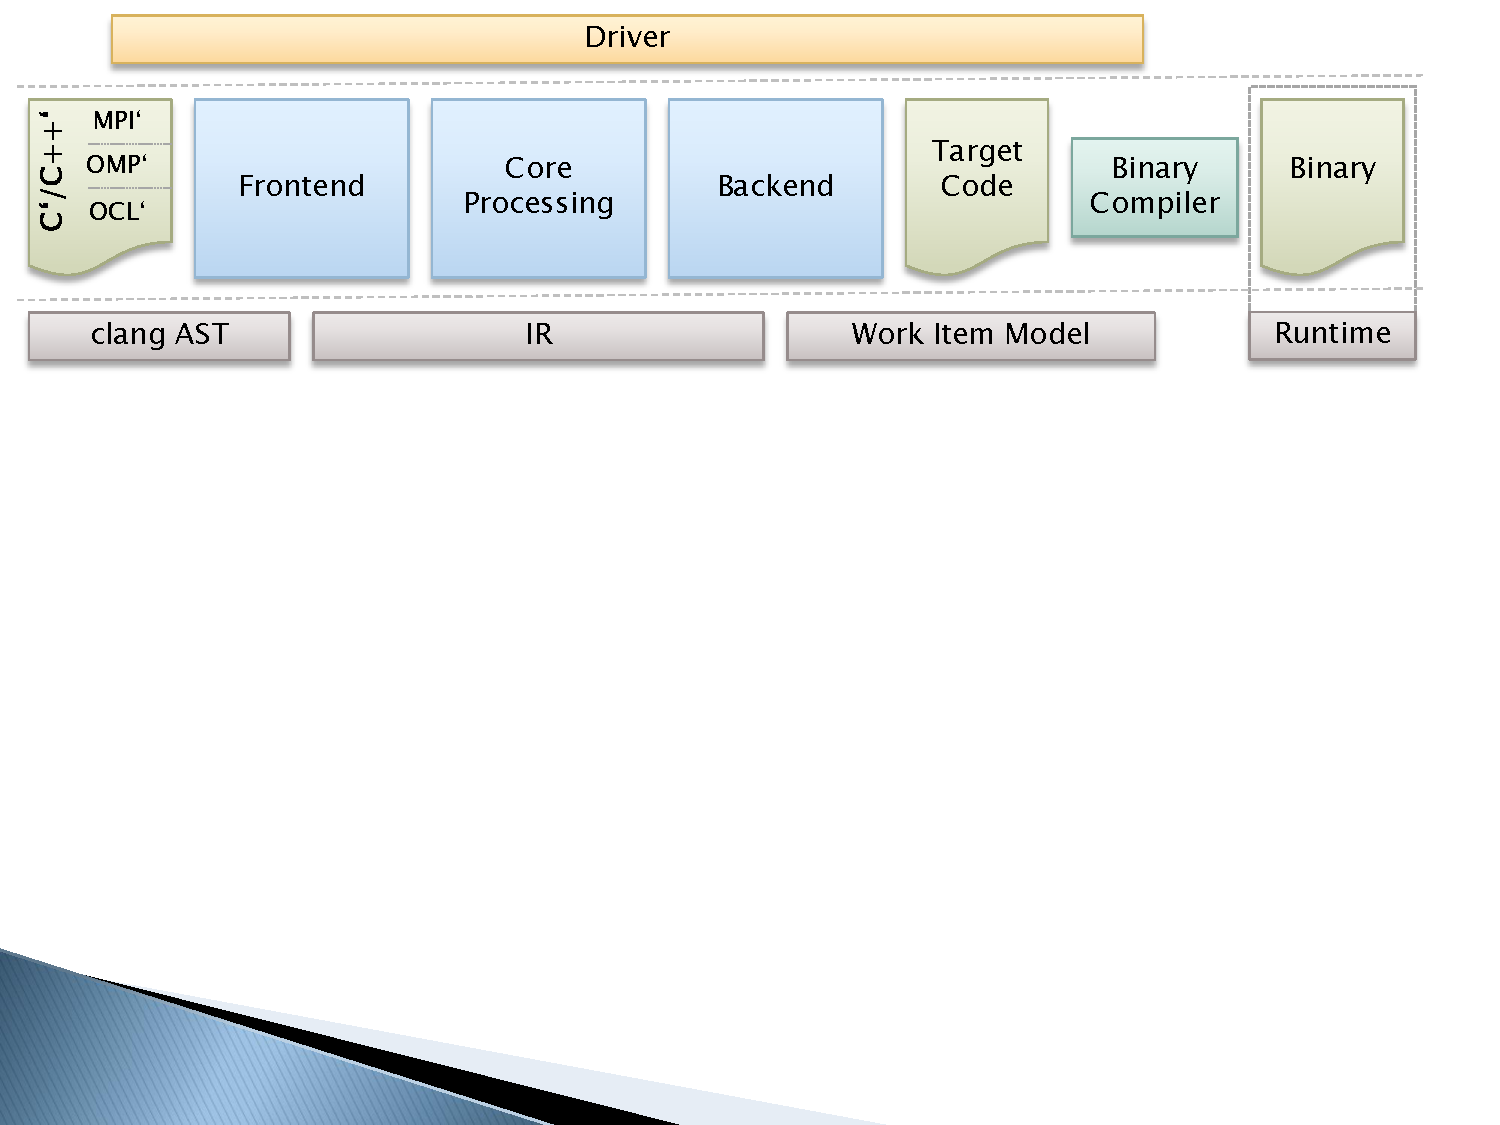
\includegraphics[width=\textwidth, trim=0 365 35 0, clip]{overview/architecture_overview.pdf}
	\caption{Overview on the Compiler's Components (blue) and the involved Program Representations (gray)}
	\label{fig:Overview.Compiler.Components}
\end{figure}


\subsubsection{Implementation Details}
From the developers point of view, the compiler is a large library of utilities.
Although there is a main executable assembling a basic pipeline of steps for
loading, processing and synthesizing codes using a flexible selection of front
and backends, in general users are encouraged to create individual executables
for their tasks. To keep executables structured, the \textit{playground} module
has been set up within the source repository. This module can be used as a
foundation for building new executables covering any required workflow. The
build environment is automatically generating build-targets for executables for
any file using the \file{cxx} extension (see \ref{sec:Infrastructure.Build}).

As a consequence of this design decision, any component / module within the
compiler has to follow the library concept by implementing some passive module
being triggered by an external control flow. To simplify the composition of
various utilities, each module should aim for providing clean interfaces for end
users. Hence, if possible, a single header file should be used. Also, all
parameters effecting the process shell be configurable at a single position,
ideally using locally allocated data structures to allow the (simple)
integration of multiple instances of the same module within a single process
instance.


\subsection{The Runtime}

\subsubsection{The Obligation}
\subsubsection{The Application Model}
\subsubsection{Important Components}
\subsubsection{Implementation Details}
Unlike the compiler, the Runtime is 

Hence, within the runtime the control flow is determined by the core
system as well as the executed program code and can not be changed. Runtime
developers can merely effect decision making processes within this
pre-determined fixed infrastructure -- which should be sufficient for most
ventures. However, in case the pre-determined ``points of influence'' are
insufficient, modifications of the framework may be conducted.


For instance,
codes to be executed using the runtime environment are required to provide
meta-information regarding the involved parallel sections. This
 



Compiler:
\begin{itemize}
  \item Common model of code (IR)
  \item Runtime common runtime model + hardware model
\end{itemize}

 using the
capabilities of the Runtime during their execution. The Runtime on the other hand provides an interface
abstracting the underlying infrastructure, hence machine.

load, parse, combine and process input
which will finally be 


To cover:
\begin{itemize}
  \item The Compiler
  \begin{itemize}
    \item The Frontend
    \item The Core
    \item The Backend
    \item Driver 
    \item Analyses
    \item Transformations
    \item Optimizers
  \end{itemize} 	
  \item The Runtime
\end{itemize}



\subsection{Overall A}


A rough overview on the projects architecture, its components and contributions.

\section{The Insieme Coding Philosophy}


\begin{itemize}
  \item Insieme Compiler vs. Insieme Runtime
  \item Compiler - tool kit to build compiler related utilities,
  transformations, analysis, \ldots
  \item Runtime - framework controlling the execution of an application;
  extended by providing alternative implementations of given functionality; flow
  of control is dictated by the runtime
  \item Point out difference: Compiler = Library = Toolkit, Runtime = Framework
\end{itemize}


State that:
\begin{itemize}
  \item Each ``component'' should represent a closed entity - usable via a simple
  user friendly interface without the requirement of modifying internal code
  \item Each component has to declare itself as a ``framework'' or ``library'' -
  define those two terms!
  \item Extendable by design - not re-design
  \item Coding standards
\end{itemize}